\begin{figure}
	\centering
	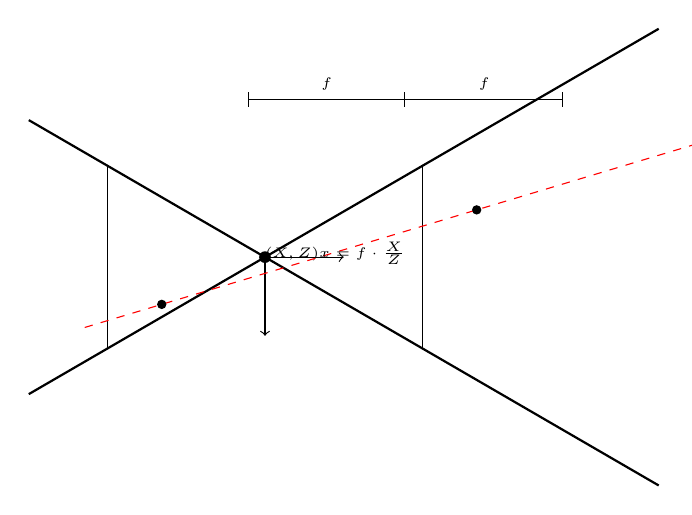
\begin{tikzpicture}
	\draw[->] (0,0) -- (1,0);
	\draw[->] (0,0) -- (0,-1);
	\tkzDefPoint(0,0){orig}
	\tkzDefPoint(1,0){z}
	\tkzDefPoint(0,-1){x}
	\tkzDefPoint(-2, -1.15){imgplane}
	\tkzDefPoint(2, -1.15){virtimgplane}
	\tkzLabelPoint[above](z){\tiny{z}}
	\tkzLabelPoint[left](x){\tiny{x}}
	\tkzLabelPoint[above=.5cm](orig){\tiny{Center of}}
	\tkzLabelPoint[above=.25cm](orig){\tiny{Projection}}
	\tkzLabelPoint[below=.7cm](imgplane){\tiny{Image Plane}}
	\tkzLabelPoint[below=.7cm](virtimgplane){\tiny{Virtual}}
	\tkzLabelPoint[below=.95cm](virtimgplane){\tiny{Image Plane}}
	\node at (0, 0) [circle, fill, inner sep=1.5pt]{};
	\draw[thick] (-3, -1.74) -- (5, 2.9);
	\draw[thick] (-3, 1.74) -- (5, -2.9);
	\draw[] (-2, 1.15) -- (-2, -1.15);
	\draw[] (2, 1.15) -- (2, -1.15);
	\tkzDefPoint(5, 1.5){P}
	\tkzLabelPoint[](P){\tiny{$(X, Z)$}}
	\node at (5, 1.5) [circle, fill, inner sep=1.2pt]{};
	\draw[color=red, dashed] (5, 1.5) -- (-3, -0.9);
	\node[] at (2, 0.6) [circle, fill, inner sep=1.2pt]{};
	\node[] at (-2, -0.6) [circle, fill, inner sep=1.2pt]{};
	\tkzDefPoint(2, 0.6){p}
	\tkzLabelPoint[](p){\tiny{$x = f \cdot \frac{X}{Z}$}}
	\draw[-|] (0, 2) -- node[above] {\tiny{$f$}} (2, 2);
	\draw[|-|] (0, 2) -- node[above] {\tiny{$f$}} (-2, 2);
	\end{tikzpicture}
	\caption{Visualization of perspective projection in the simplified two dimensional case.
		The camera with focal length $f$ is located at the origin.
		The point $(X, Z)$ is projected onto the (virtual) image plane via perspective projection.
		The resulting x coordinate is $x = \pm f \cdot \frac{X}{Z}$.}
	\label{fig:camera-projection-setup}
\end{figure}